\documentclass{beamer}
\usepackage[utf8]{inputenc}
\usepackage{graphicx}
\usetheme{Warsaw}
\usecolortheme{seahorse}

\title{Genalice/SciLifeLab NGI Applications - testing NA12878, in progress }
\author{Szilveszter Juhos, Max Käller}
\institute{SciLifeLab}
\date{1st Sep. 2016 }
\begin{document}
\frame{\titlepage}
			  
\begin{frame}
	\frametitle{NA12878 truth set}
	\begin{block}{Platinum reads from Illumina (NA12878 ERR194147) }
	There are many truth sets hanging around
	\end{block} 
	\begin{itemize}
		\item GIAB (multiple platforms)
		\item Illumina Platinum 
		\item 1000 Genomes VCF (1KG)
	\end{itemize}
VCFLIB https://github.com/vcflib/vcflib to get stats and set operations

	\begin{block}{call set that contains Genalice only variants}
	$ Genalice \setminus (GIAB \cup Platinum \cup 1KG) $
	\end{block}
\end{frame}

\begin{frame}
	\begin{itemize}
		\item Considering SNPs only now
		\item $\sim$200K SNPs filtered as unique to Genalice
		\item Looking at alignments (chr20 only) with the Genalice IGV jar
		\item surveying only SNPs that are different from truth sets
	\end{itemize}
	\begin{block}{IGV plugin}
	Browsing GAR files is much faster than BAMs (i7 Dell laptop)

	Upper track: Genalice GAR

	Lower track: BWA alignment
	\end{block}
\end{frame}

\begin{frame}
\frametitle{False positives at deletions}
\center{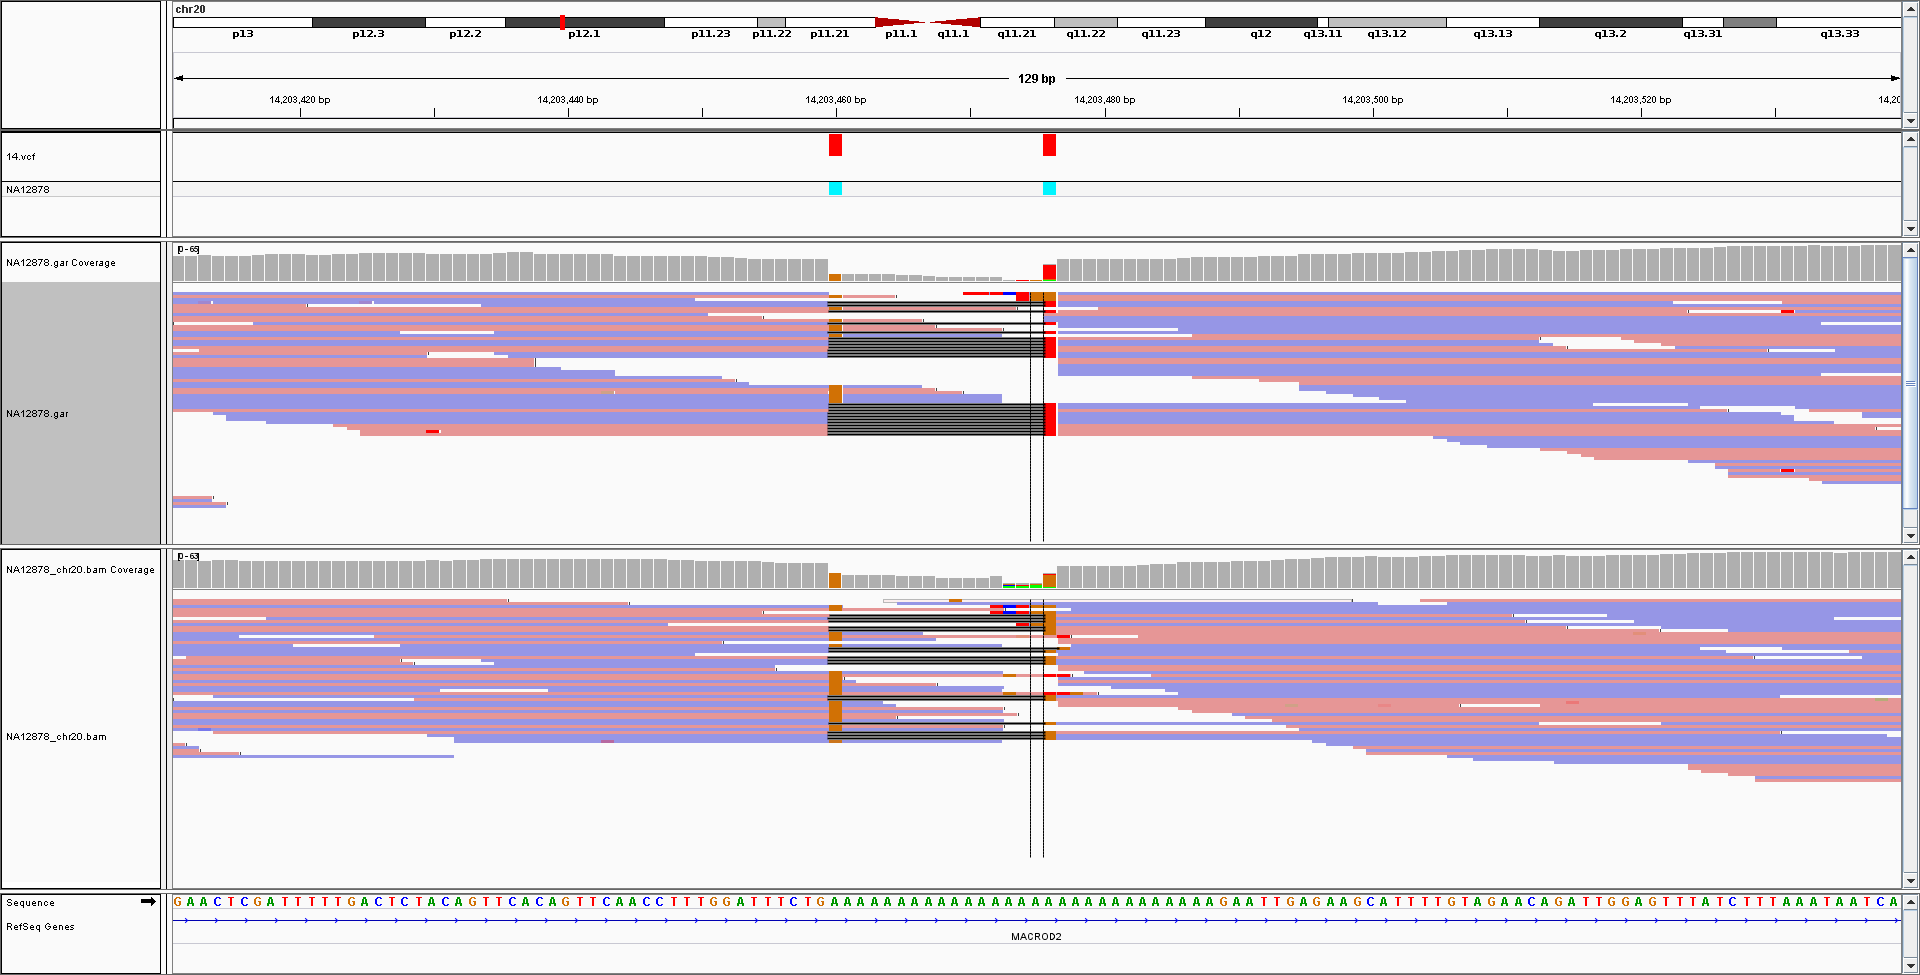
\includegraphics[width=1.0\linewidth]{igv_deletion.png}}
Can be filtered: have to consider deletions
\end{frame}

\begin{frame}
\frametitle{False positives at low complexity parts}
\center{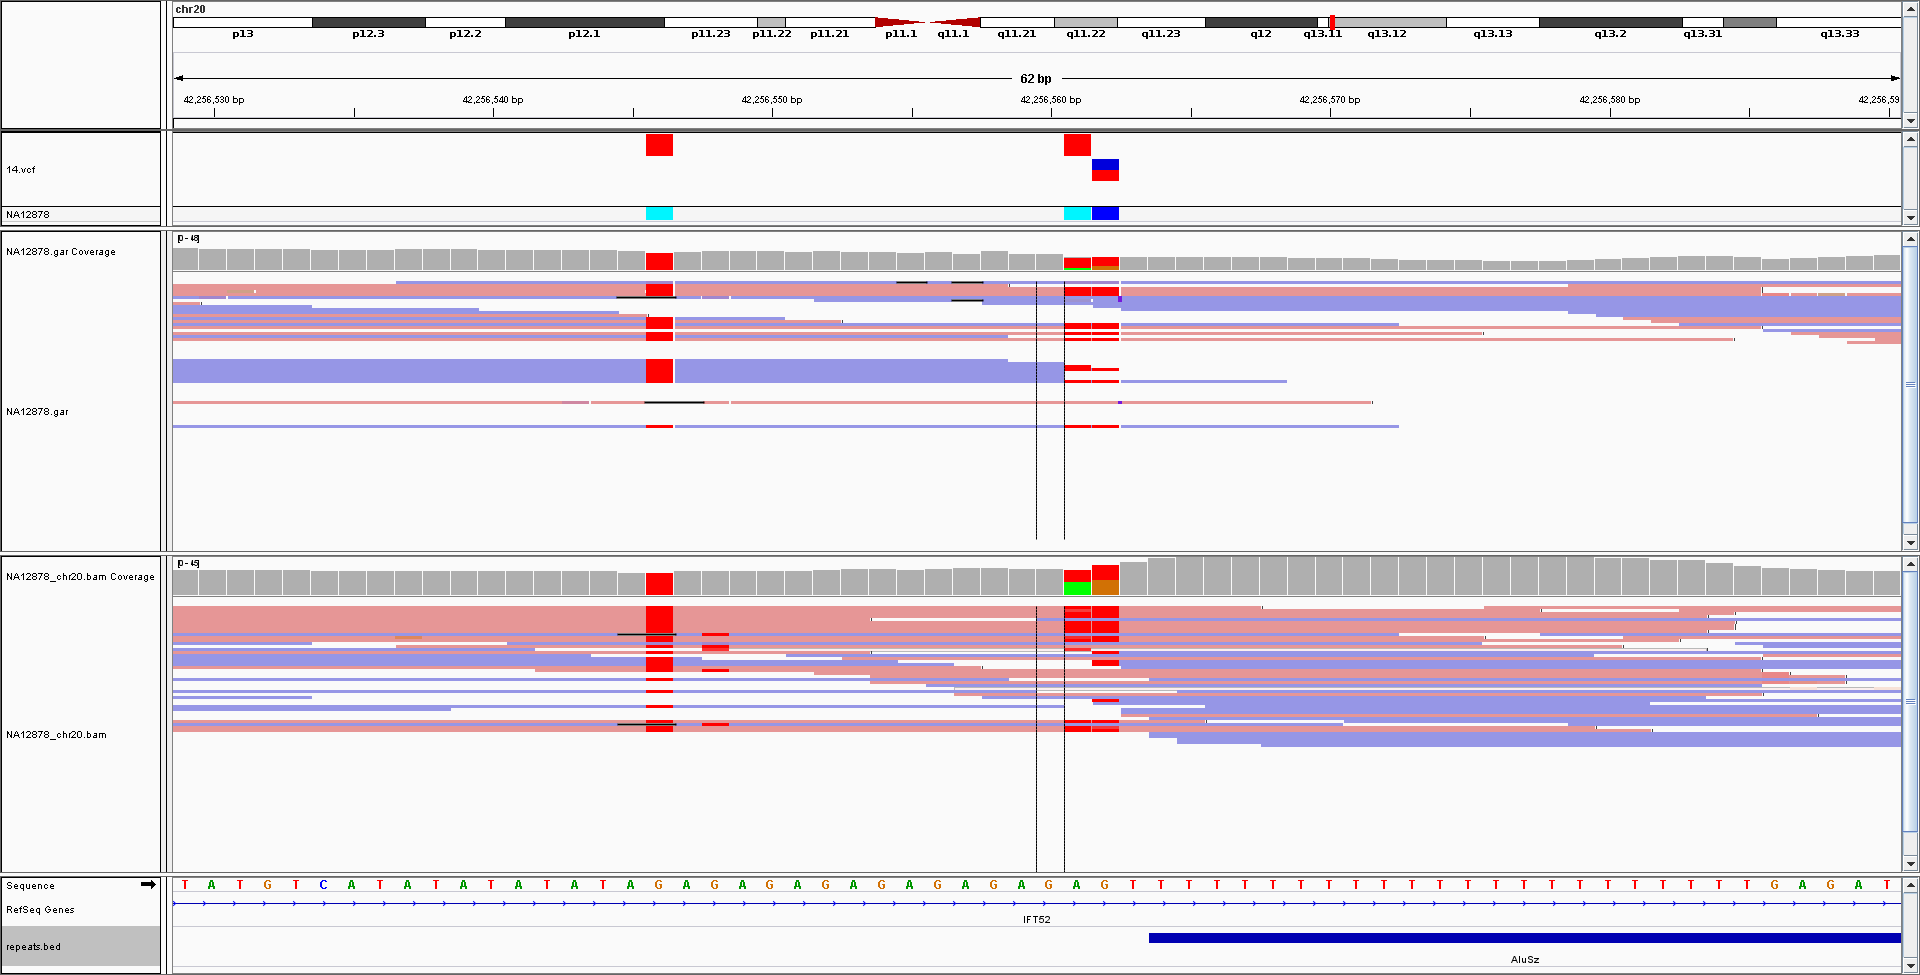
\includegraphics[width=1.0\linewidth]{igv_GAGA.png}}
Can be filtered though not that straightforward
\end{frame}

\begin{frame}
\frametitle{False positives at GC-rich regions}
\center{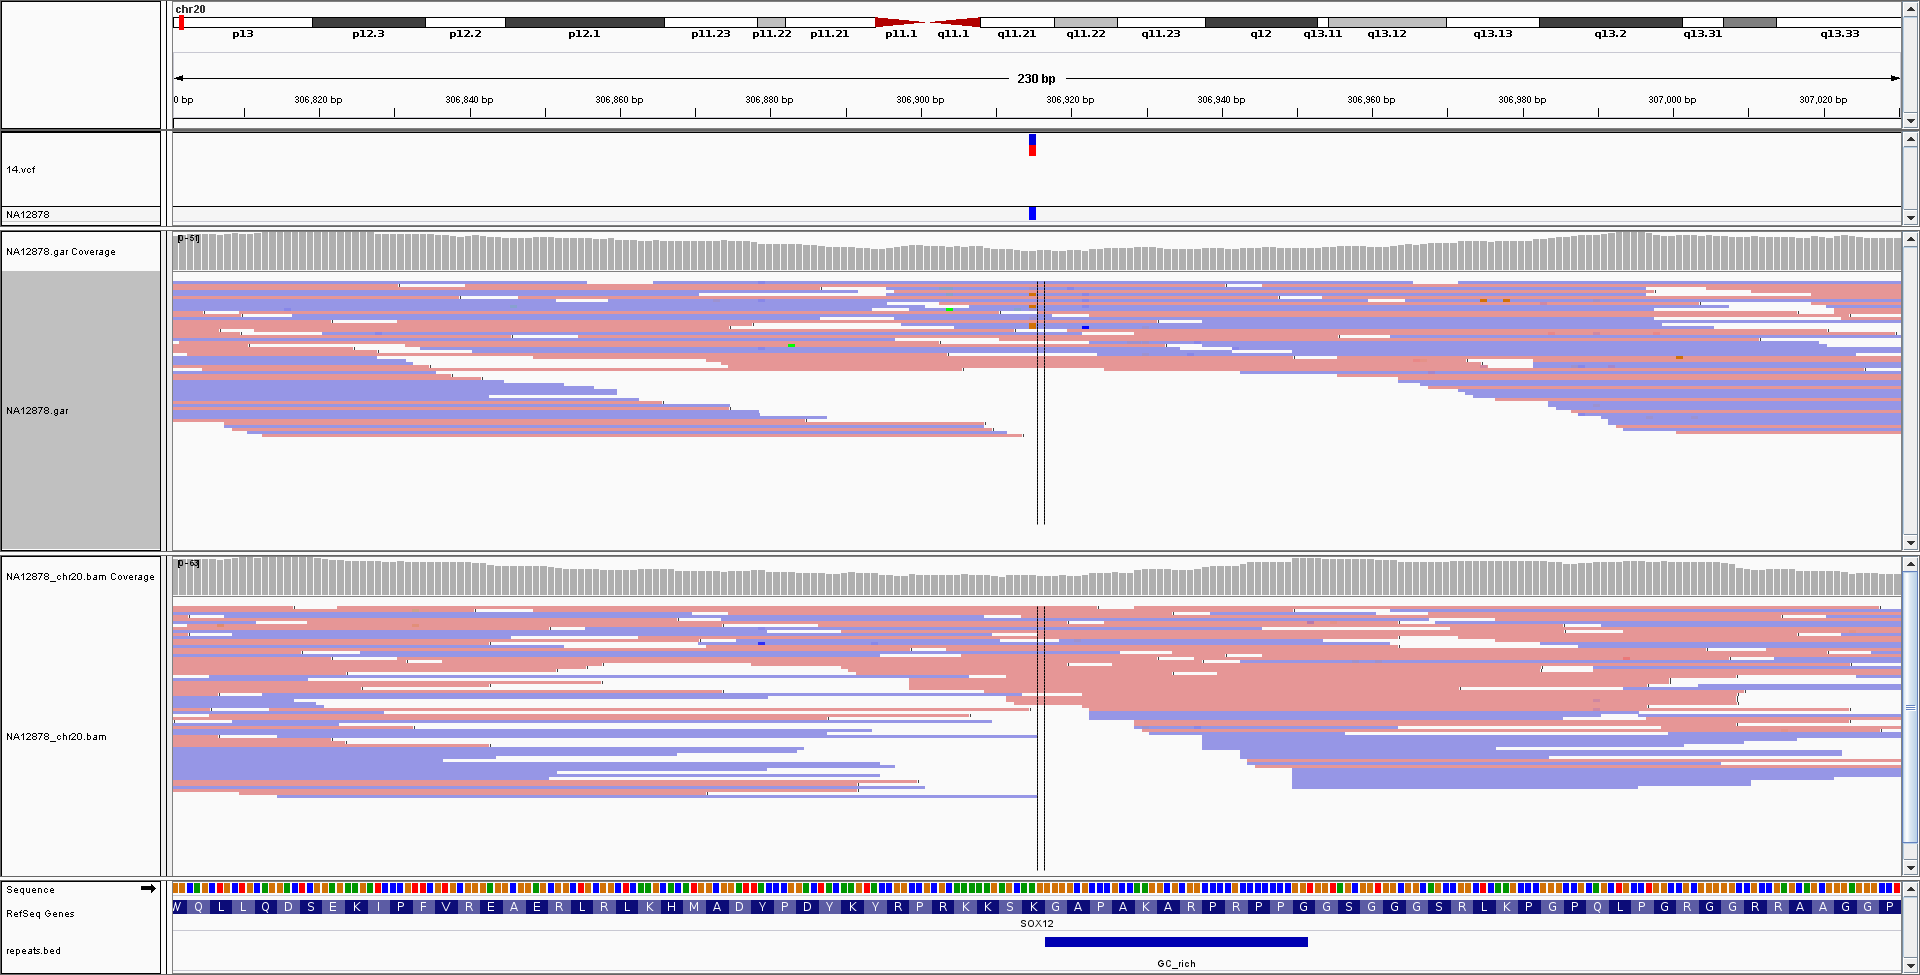
\includegraphics[width=1.0\linewidth]{igv_GC-rich.png}}
Tough, but expert can filter it out
\end{frame}

\begin{frame}
\frametitle{False positives at repeats}
\center{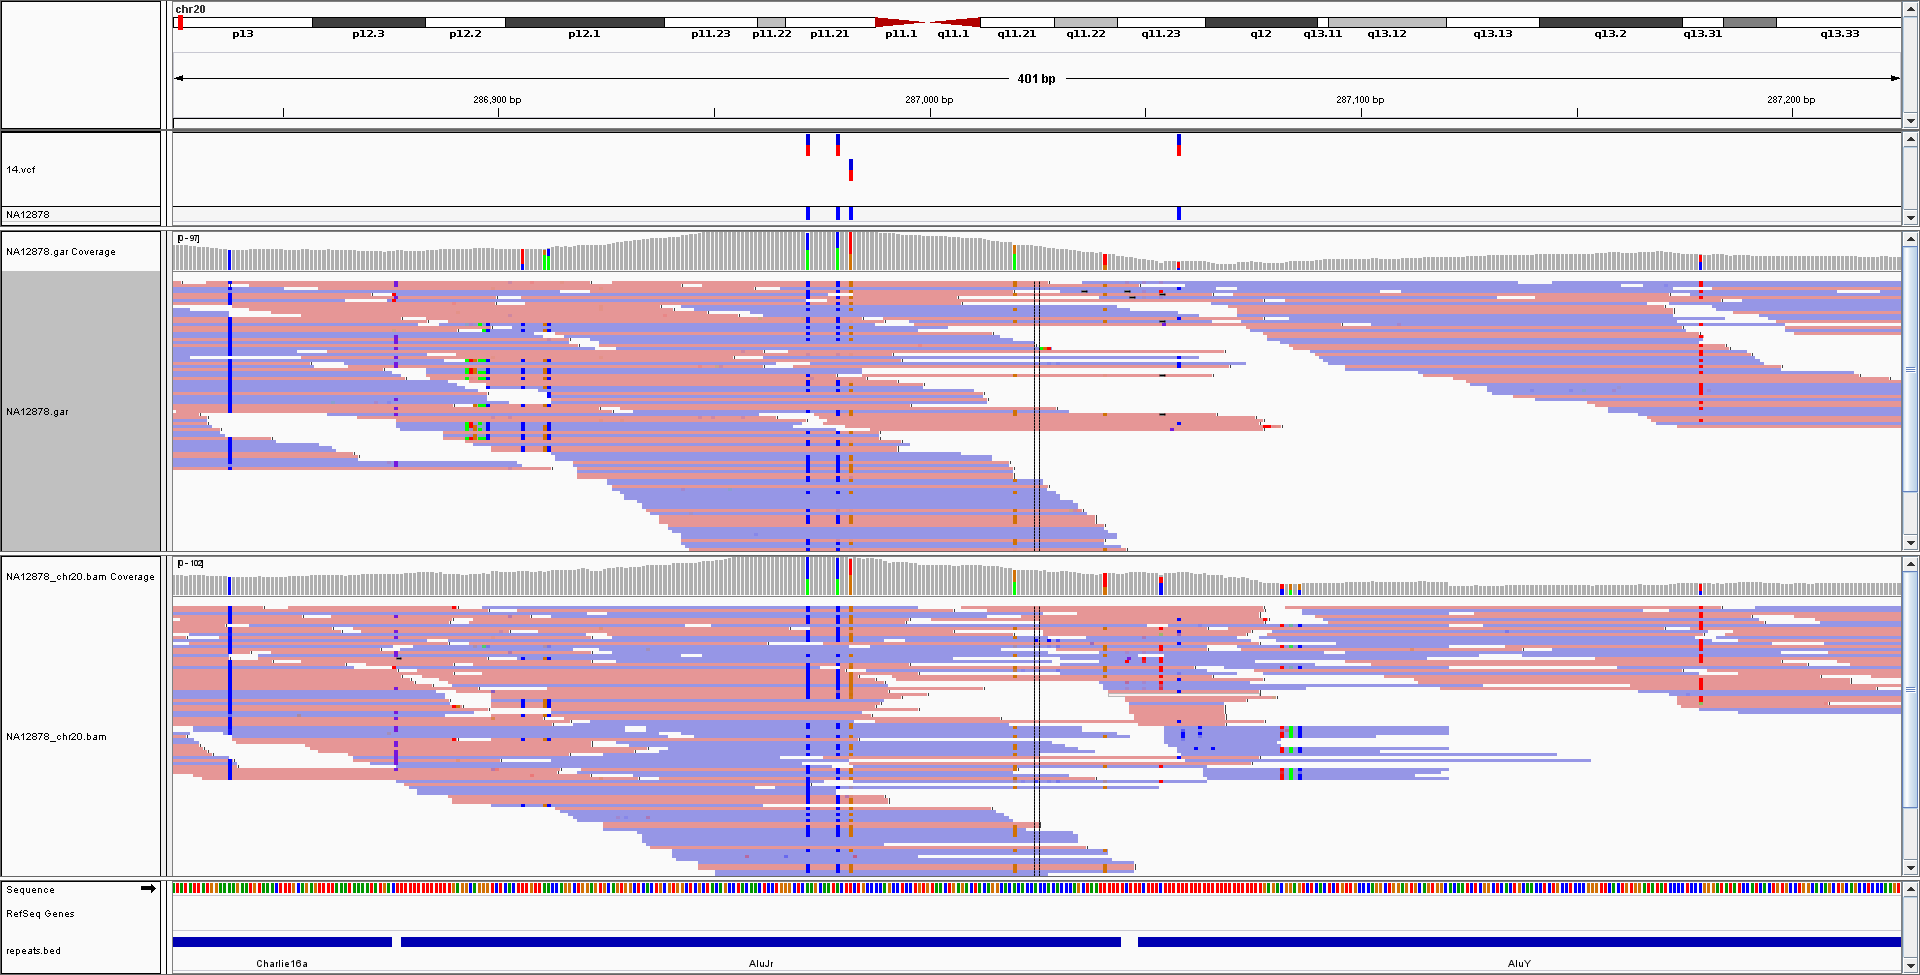
\includegraphics[width=1.0\linewidth]{igv_Alu.png}}
Can be filtered out also
\end{frame}

\begin{frame}
\frametitle{False positives at repeats}
\center{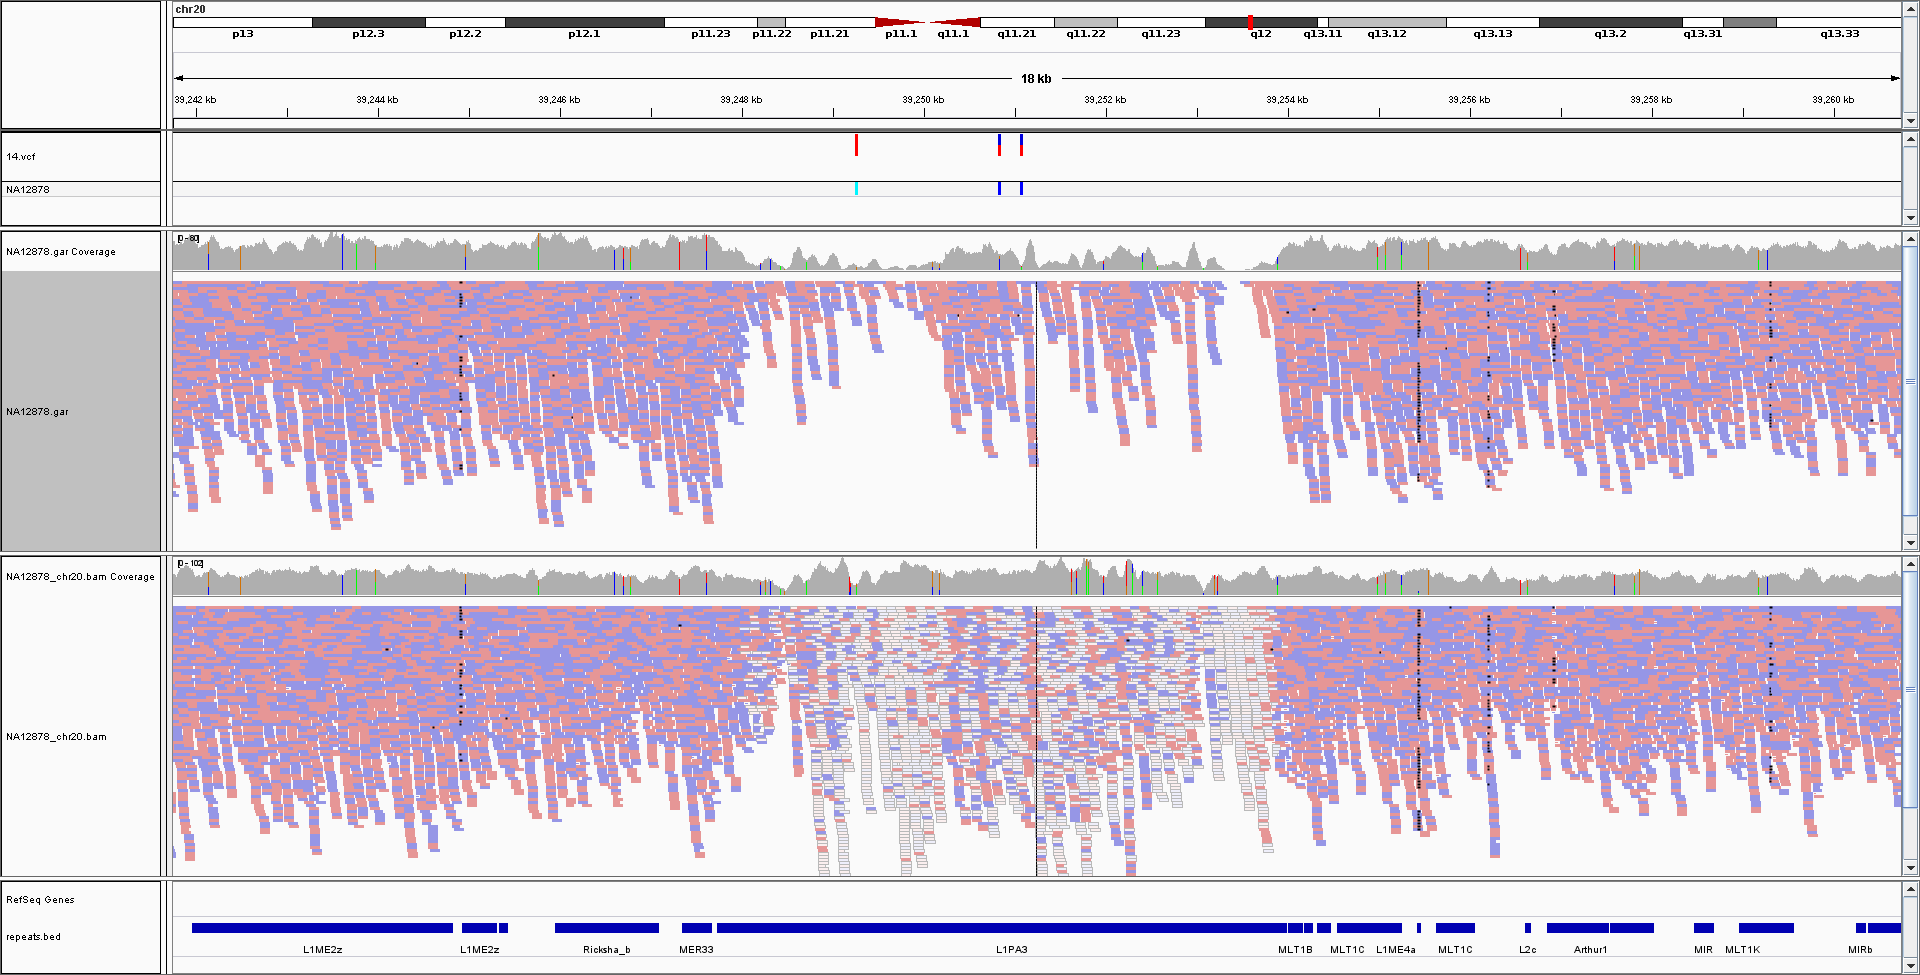
\includegraphics[width=1.0\linewidth]{igv_L1PA3.png}}
Reads mapping to multiple locations actually can help to throw out false positives
\end{frame}

\begin{frame}
\frametitle{Nastly regions like MHC}
\center{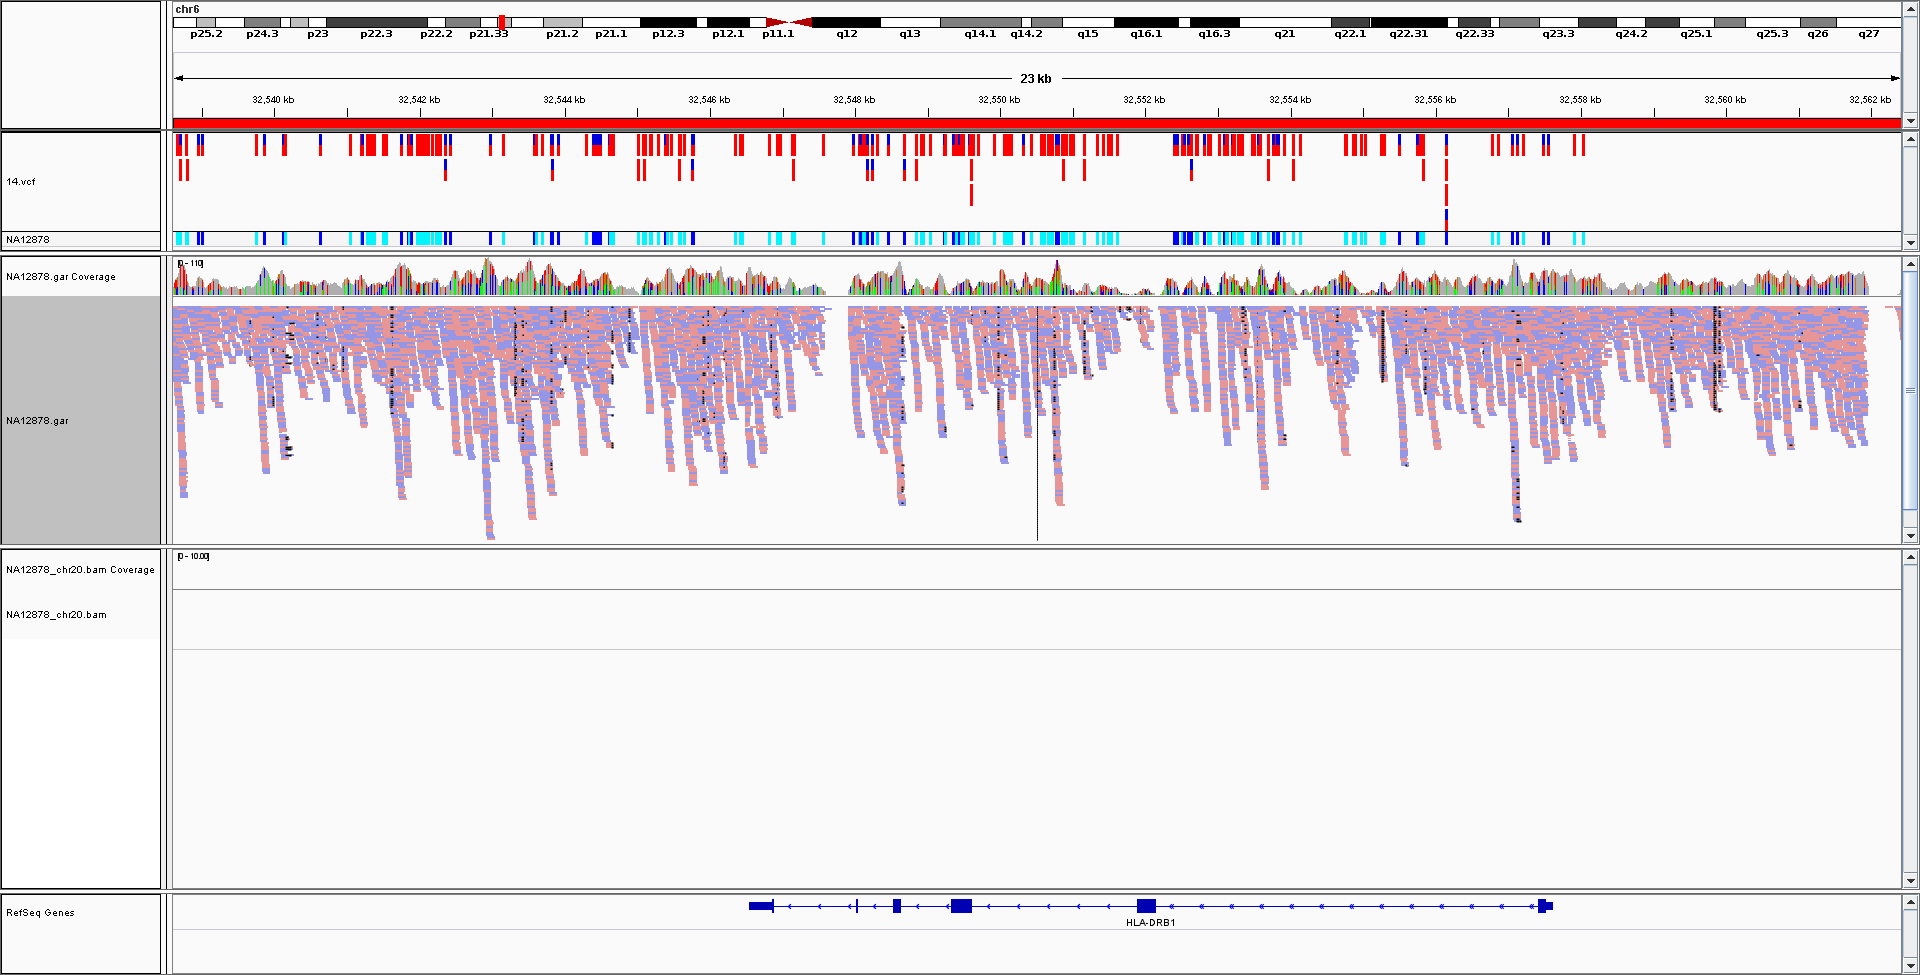
\includegraphics[width=1.0\linewidth]{igv_DRB1.png}}
These parts of the genome have to be treated as different beasts
\end{frame}

\begin{frame}
\frametitle{Real positives?}
\center{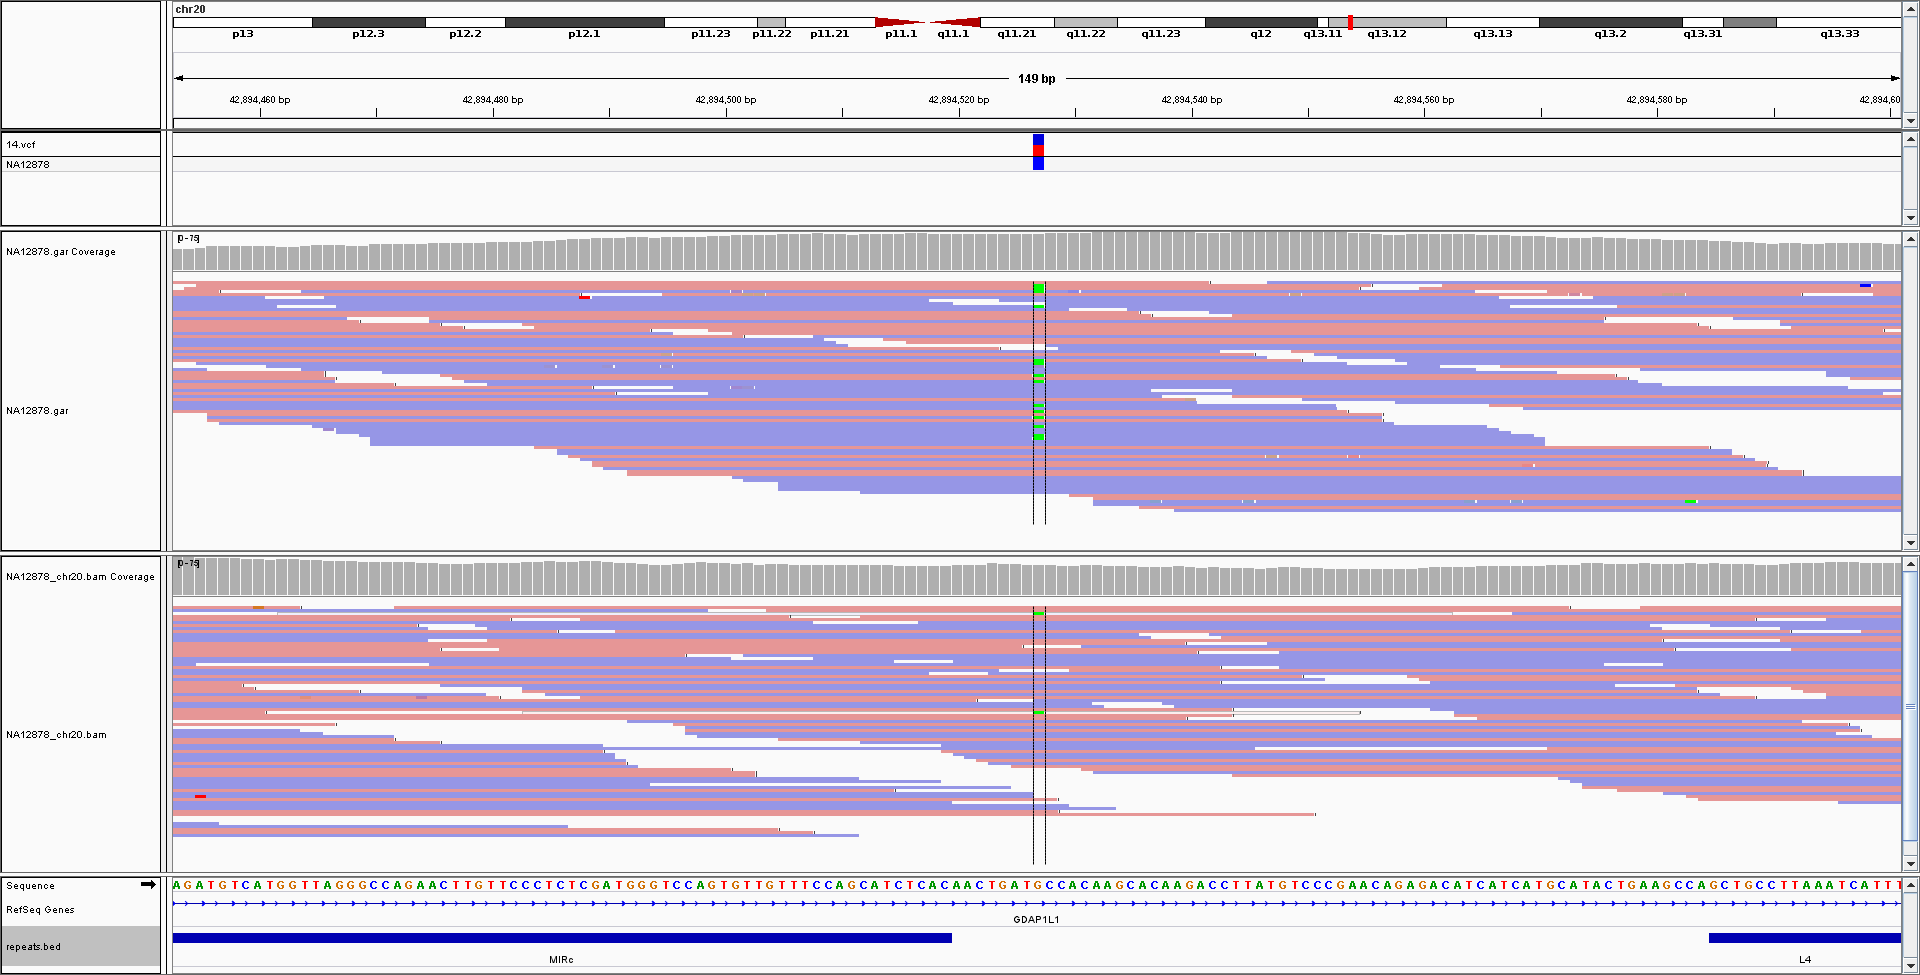
\includegraphics[width=1.0\linewidth]{igv_GDAP1L1.png}}
\end{frame}

\end{document}
